\chapter{Evaluation}\label{ch:evaluation}
Evaluation of the Laha framework involves deploying reference Laha-compliant DSNs, validating the data collected from the reference implementations, and then comparing and contrasting various metrics for each of the stated goals. Metrics were collected during a set of experiments for each of the Laha reference implementations in summer 2019.

The following sections describe my plans for deployment of reference implementations, data validation, evaluating the main goals of the Laha framework, and evaluating the tertiary goals of the Laha framework.

\section{Deploy Laha reference implementations on test sites}\label{sec:deploy-laha-reference-implementations-on-test-sites}
Both the OPQ and Lokahi reference implementations were deployed to test sites where validated data collection took place. The following sections describe the reference implementation deployments in detail.

\subsection{OPQ Reference Deployment}\label{subsec:opq-reference-deployment}
Fifteen Laha-compliant OPQ Boxes were deployed over the UH Manoa microgrid during the Summer of 2019.

The placement strategy I utilized aimed to maximize collecting distributed PQ events by placing sensors on the same electrical lines. We also considered placing Boxes in locations co-located with sensitive or demanding electrical equipment in the hopes of seeing PQ events generated from this equipment. Finally, we considered data access in terms of network availability and ground truth availability. Working with my colleagues and the Office of Energy Management, I selected the locations for the campus wide deployment. Table \ref{table:OpqDeployment} displays the details of the UH Manoa campus deployment and justifications for choosing those locations.
The placement strategy I utilized aimed to maximize collecting distributed PQ events by placing sensors on the same electrical lines. We also considered placing Boxes in locations co-located with sensitive or demanding electrical equipment in the hopes of seeing PQ events generated from this equipment. Finally, we considered data access in terms of network availability and ground truth availability. Working with my colleagues and the Office of Energy Management, I selected the locations for the campus wide deployment. Table \ref{table:OpqDeployment} displays the details of the UH Manoa campus deployment and justifications for choosing those locations.

\begin{table}[H]
	\centering
	\caption{OPQ Deployment}
	\begin{tabularx}{\textwidth}{lllX}
		\toprule
		\textbf{Box} & \textbf{Location} & \textbf{Coordinates} & \textbf{Description} \\
		\midrule
		1000 & POST (CSDL) & -157.816237,21.297438 & Same line as 1002, 1009, 1010, 1013. Sensitive computer equipment. \\
		1001 & Hamilton (Basement 3F) & -157.816173,21.300332 & Same line as 1008. Ease of access. \\
		1002 & POST (ICSpace) & -157.826327,21.30046 & Same line as 1000, 1009, 1010, 1013. Sensitive computer equipment.   \\
		1003 & IT Building & -157.826327,21.30046 & Same line as 1004. Sensitive computer equipment. \\
		1004 & Building 37 & -157.817821,21.298732 & Same line as 1003. LAVA Lab. \\
		1005 & Parking Structure (Phase II) & -157.819234, 21.296042 & Same line as 1011, 1012. Proximity to PV. \\
		1006 & Frog I & -157.823122,21.298050 & Same line as 1007, 1014. Proximity to PV. PV ground truth access. \\
		1007 & Frog II & -157.822819,21.298046 & Same line as 1006, 1014. Proximity to PV. PV ground truth access.  \\
		1008 & Ag. Engineering & -157.816107,21.301564 & Same line as 1001. Known PQ issues. \\
		1009 & Watanabe & -157.815817,21.298351 & Same line as 1000, 1002, 1010, 1013. Sensitive physics instruments. \\
		1010 & Holmes & -157.816104,21.297011 & Same line as 1000, 1002, 1009, 1013. Machining shops and electronic equipment. \\
		1011 & Parking Structure (Phase I) & -157.817430,21.295338 & Same line as 1005, 1012. Proximity to PV. \\
		1012 & Law Library & -157.817361,21.296328 & Same line as 1005, 1011. \\
		1013  & Kennedy Theater & -157.815225,21.299282 & Same line as 1000, 1002, 1009, 1010. Demanding electronic equipment. \\
		1014 & Sinclair Library & -157.820499,21.298475 & Same line as 1006, 1007. \\
		1015 & Architecture Portables & -157.813644,21.301092 & Edge of campus. Portable buildings. \\
		\bottomrule
	\end{tabularx}
	\label{table:OpqDeployment}
\end{table}
Determination of electrical lines was aided by the UH Manoa electrical blueprint as displayed in Figure~\ref{fig:UhGridTopo}.

\begin{figure}
	\centering
	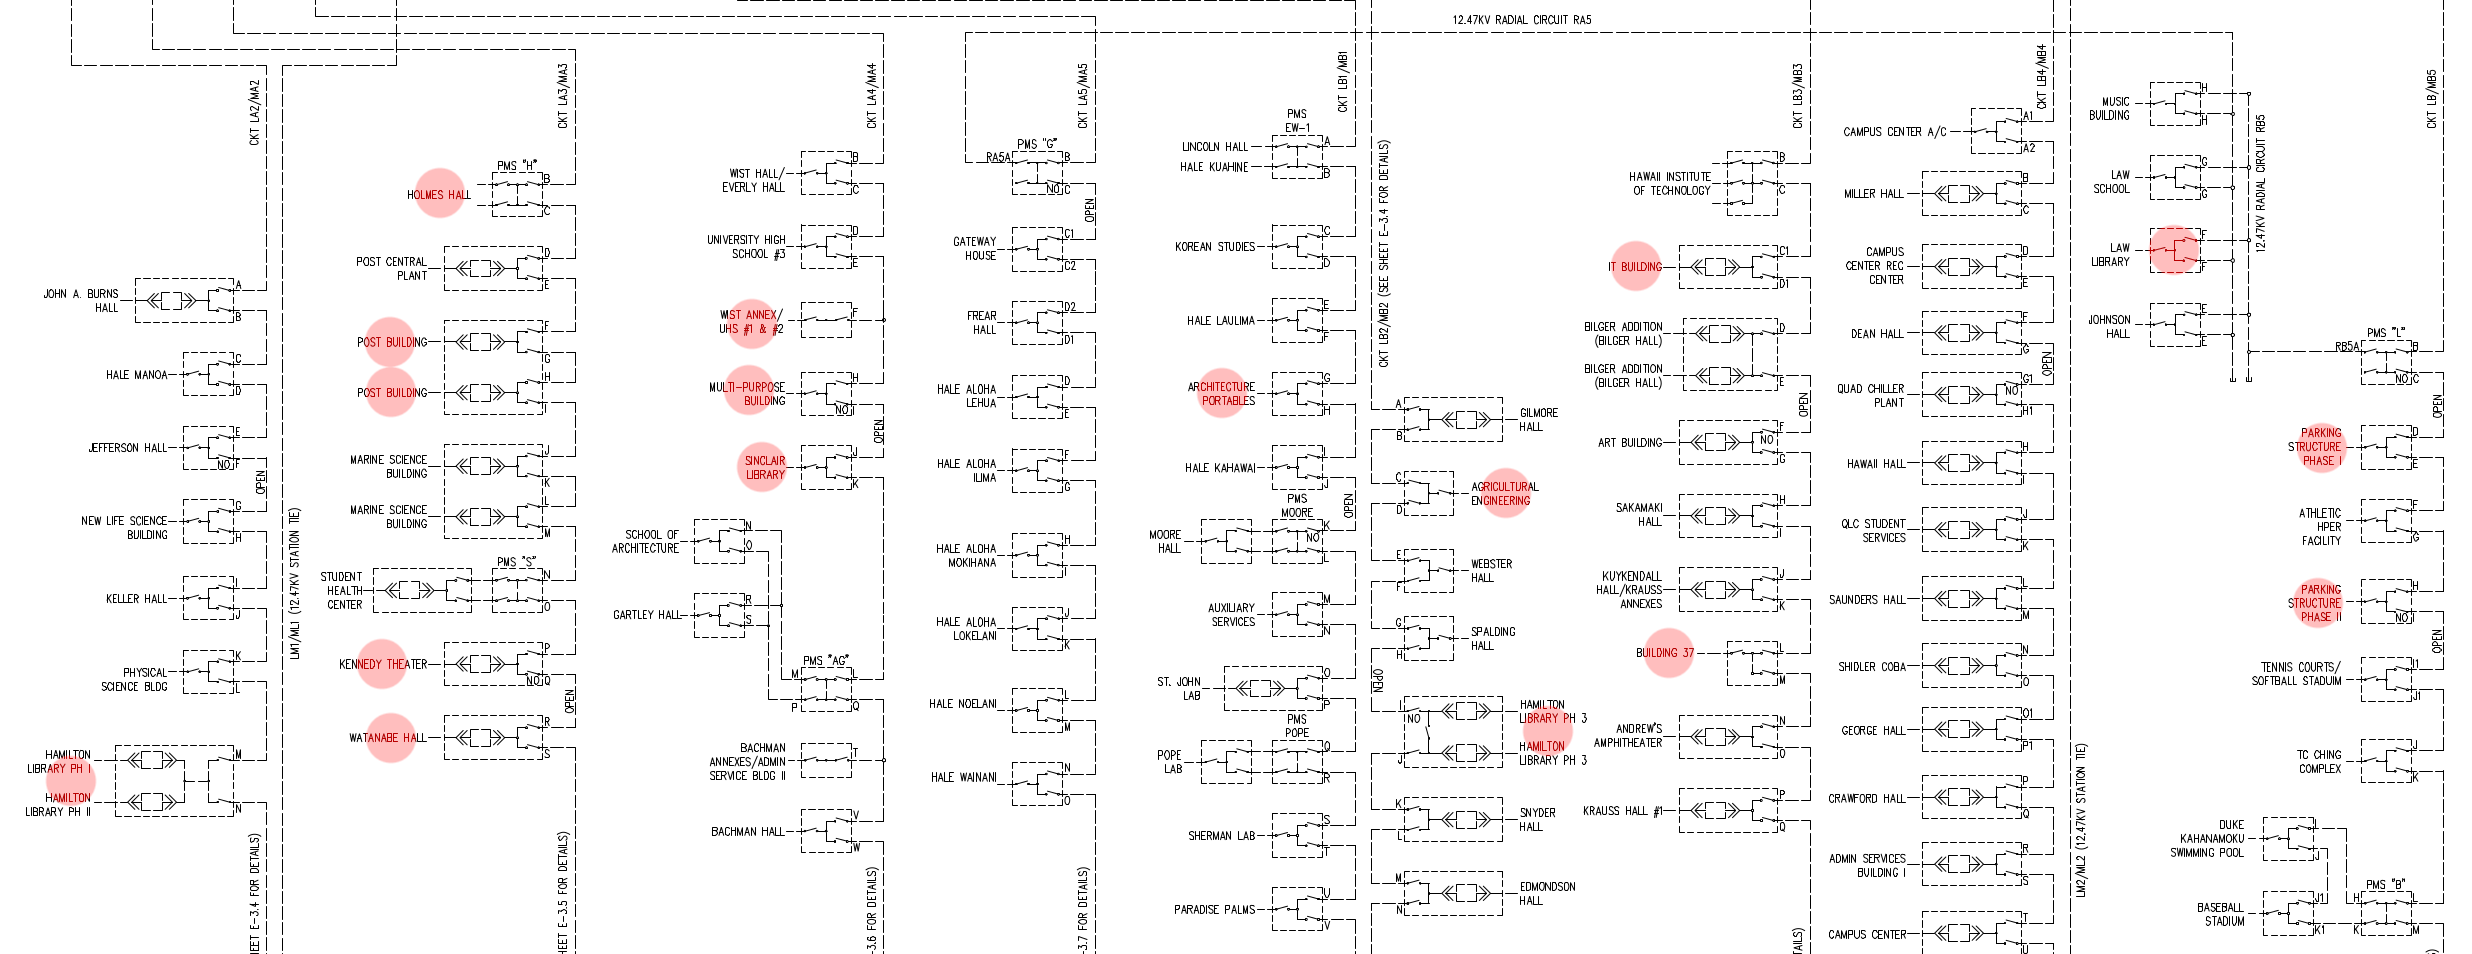
\includegraphics[width=\linewidth]{figures/uh_thesis_depoyment_v1.png}
	\caption{UH Deployment Grid Topology}
	\label{fig:UhGridTopo}
\end{figure}

A graphical representation showing the complete coverage of Boxes on the UH Manoa microgrid is displayed in Figure \ref{fig:UhDeploy}.

\begin{figure}
	\centering
	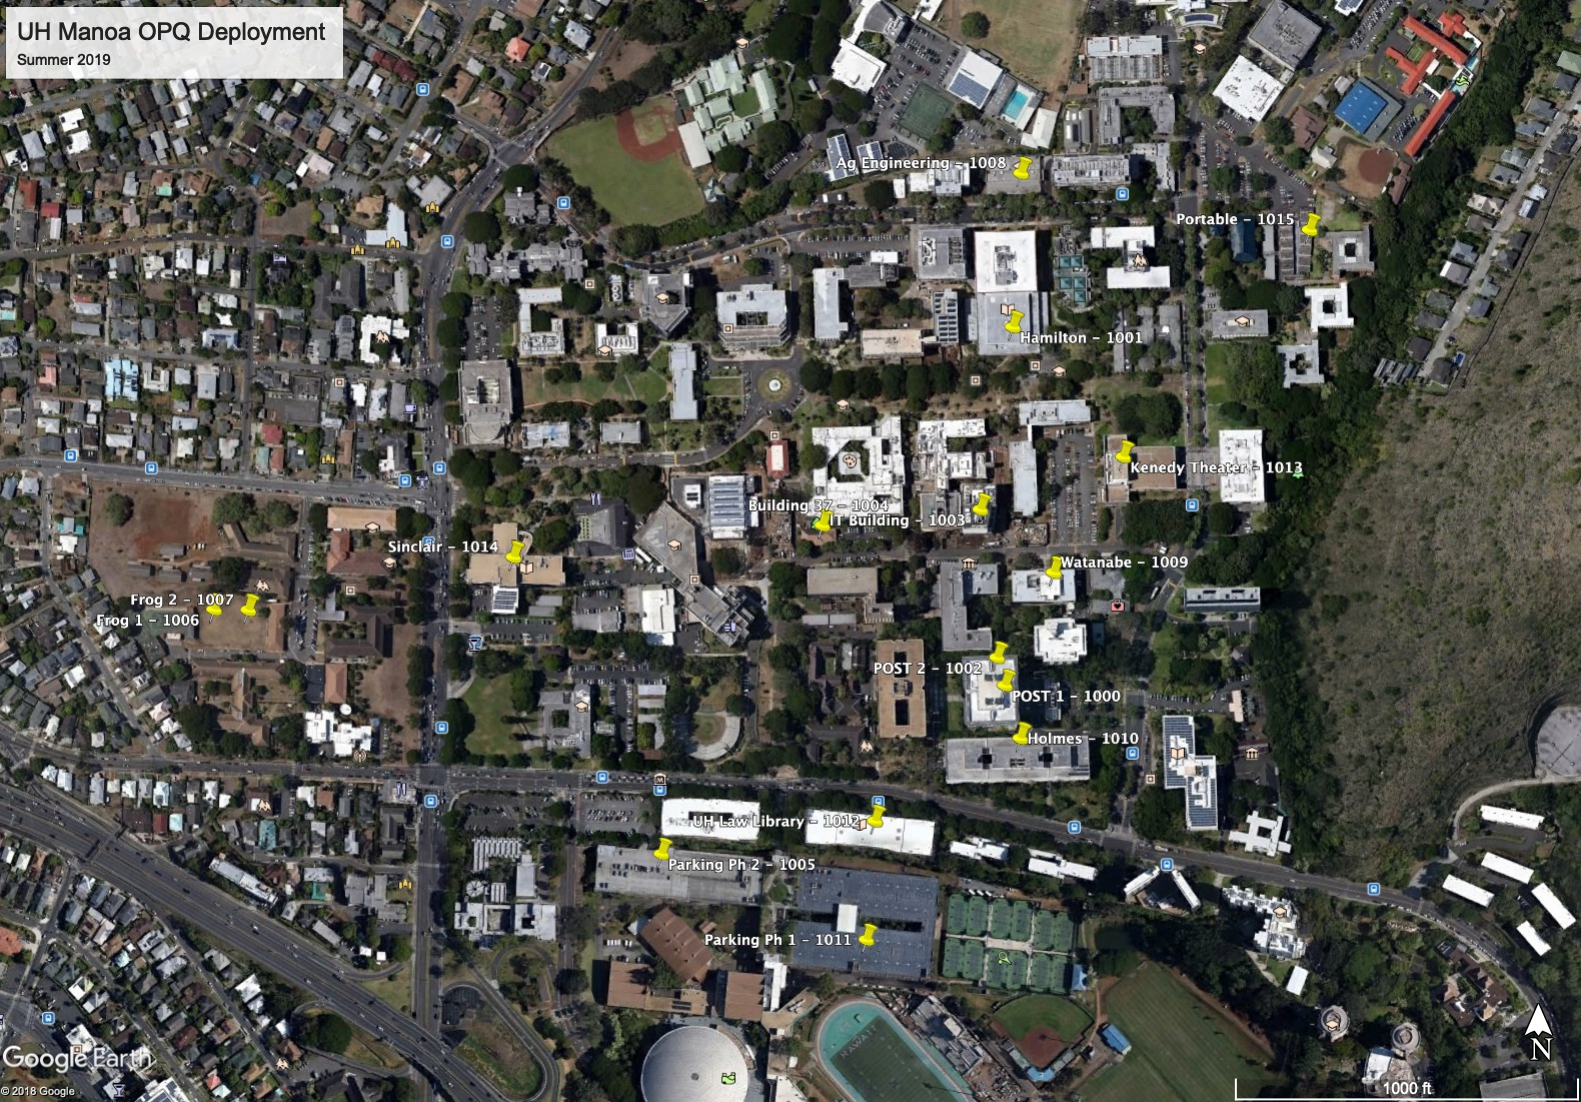
\includegraphics[width=\linewidth]{figures/deploy.jpg}
	\caption{UH Deployment}
	\label{fig:UhDeploy}
\end{figure}

All devices were placed in a location that had access to UH Manoa's wireless network. As soon as they were installed, they started transmitting PQ data for that location.

\subsection{Lokahi Reference Deployment}\label{subsec:lokahi-reference-deployment}
%TODO

\section{Validate data collected by Laha deployment}\label{sec:validate-data-collected-by-laha-deployment}
Data from both experimental deployments were validated against ground truth data. In the OPQ deployment, ground truth is provided by UH meters installed at the main of each building. In the Lokahi deployment, ground truth was provided by high-end calibrated microphones.

\subsection{Validate data collected by OPQ deployment}\label{subsec:validate-data-collected-by-opq-deployment}

Ground truth for the UH Manoa microgrid deployment is provided by UH system installed power meters. These meters were installed at the main of most buildings and can provide ground truth for Voltage, Frequency, and THD trends, as well as provide a maximum bounds of these features enabling me to determine if the incidents we see in OPQ would have been seen by the UH meters.

The UH meters provide data trends for Voltage, Frequency, and THD in rolled-up one minute windows. Each window provides descriptive statistics for the feature it is measuring including minimum, maximum, average, and standard deviation of the feature values during the one minute window. By using the minimum and maximum values, I was able to provide upper and lower bounds for whether or not the PQ incidents we observed were valid or not.

As an example, if an Incident is created by Mauka with a Voltage sag down to 110V, then I would expect the nearest ground truth meter to also have a minimum Voltage value near 110V for the same time window. If the minimum value from the UH meter does not show a Voltage drop, then we know that Mauka identified a false positive.

I have written a separate service for OPQ called the ``ground-truth-daemon". The role of this daemon is to query the UH Manoa metering HTTP API once per hour and retrieve the previous hours worth of data for all ground truth meters co-located with an OPQ Box or near an OPQ Box. The descriptive statistics along with the meter metadata are stored in MongoDB so that OPQ data can be compared to the ground truth data to identify false positives and false negatives. The ground truth data model was described in Table~\ref{table:ground_truth}.

Since one of the core tenants of Laha is to throw away uninteresting data, we need to store all ground truth data in an effort to identify false negatives.

Two types of validation are performed. First, we compared measurements and trends collected by OPQ to trend data collected by the UH meters. Then, we generated a report that showed the percent different between the two sets of meters. Any differences larger than 5 percent are recorded.

The second type of validation I performed was checking the bounds of Mauka generated Incidents. When a Voltage Incident is generated, the sag or swell is compared against the minimum and maximum ground truth trends. Differences larger than 5 percent were recorded. Validation for Frequency and THD was performed in a similar way.

\section{Use Laha deployments to evaluate the main goals of the framework}\label{sec:use-laha-deployments-to-evaluate-the-main-goals-of-the-framework}
The Laha deployments for both OPQ and Lokahi were used to evaluate each of the main goals this framework claims to provide. Namely that Laha is a generally useful framework representation for DSNs. Second, Laha provides the ability to turn primitive sensor data into actionable data and insights. Third, Laha's tiered management of sensor data provides metrics on maximum bounds for storage requirements and graceful degradation of DSN performance.

Each deployment requires different techniques for performing evaluation.

In the OPQ deployment, OPQBoxes are deployed and co-located with industry standard, calibrated, reference sensors. Each of these sensors cost thousands to obtain and install, collect all the data all the time, and can only be connected to the power main as it enters a building. These sensors provide a means for verifying signals received or not received by OPQ, as well as confirming long term trend data. I have been provided access to these sensors and stored data via the Office of Energy Management at UH Manoa. The data is accessible via an HTTP API. The Office of Energy Management at UH Manoa has also provided the full schematics for the UH power grid. This was used as a ground truth for topology estimates and distributed signal analysis. OPQBoxes are placed in strategic locations on the UH Manoa campus specifically in order to evaluate the distributed nature of PQ signals. For example, OPQBoxes are placed on the same electrical lines as well as separate electrical lines to observe how PQ signals travel through an electrical grid.

In the Lokahi deployment, I had the opportunity to generate infrasound signals using a calibrated infrasound source \cite{park2009rotary}.. The source can be tuned to produce infrasound at configurable frequencies and amplitudes. The source works by attaching a variable pitch propeller to an electric motor that can be driven by a waveform generator. The source can generate signals that can be observed at large stand off distances, over tens of kilometers. Similar to the OPQ deployment, sensors within the Lokahi deployment were co-located with industry standard, calibrated, infrasound sensors. These sensors can provide a metric of signals that were correctly observed, incorrectly observed, or not observed at all by the Lokahi deployment. Further, infrasound itself is characterized quite well by various geophysical equations. These equations can be used to predict if sensors deployed in the Lokahi deployment are likely to observe generated infrasound signals.

Evaluation of the main goals of this network are provided in the following sections.

\subsection{Evaluation of the Generality of this Framework}\label{subsec:evaluation-of-the-generality-of-this-framework}
I claim that the Laha framework is useful and general enough to be applied to DSNs in different domains. To test this, I designed, developed, and deployed two DSNs. The first OPQ, measures distributed PQ signals on the electrical grid. The second, Lokahi, observes infrasound signals traveling through the atmosphere.

To evaluate the generality of the Laha design, I provided metrics for whether or not each deployment is able to fulfill the goals of the given network.

I expect the PQ network, OPQ, to be able to detect and classify common PQ issues. I expect OPQ to observe voltage dips, voltages swells, frequency dips, frequency swells, transients, and high levels of THD. A count of these signals were kept and compared against industry standard PQ meters co-located with each sensor. By comparing these signals to the ground truth, we were able to tabulate a number of false positives and false negatives. In order to be considered effective, I would expect to be able to classify each of these common PQ signals, collect a set of each of the PQ signals while maintaining a low number of false positives and false negatives as compared to the industry standard sensors. In general, a negative result here would be not being able to detect PQ signals of a specific type or having a high number of false positives or false negatives.

Further, another stated goal of OPQ is to detect and classify distributed PQ incidents. That is, PQ signals that are observed by more than one sensor in situations where OPQ sensors are not co-located. First, I evaluated if OPQ is capable of detecting distributed PQ signals. I expect OPQ to at least observe one distributed signal during the test deployment, but would not be surprised to see many. By working with the Office for Energy Management at UH Manoa, I used a list of known PQ source events along with signals collected by OPQ and the industry standard sensors to provide a list of false positives and false negatives for the number of distributed PQ incidents observed by OPQ.

I expect the infrasound network, Lokahi, to be able to securely detect and report on infrasound incidents from a large collection of heterogeneous smartphone based infrasound sensors. This network prioritizes availability and security even in the face of network issues or no network at all. I claim that Laha is a useful framework for a DSN such as this and evaluated if Laha is able to meet the goals of this network.

To evaluate the effectiveness of Laha as implemented by Lokahi, I deployed 50 heterogeneous Lokahi smartphone sensors at predetermined distances from a calibrated infrasound source. I then used the calibrated infrasound source to generate infrasound signals of different amplitudes and frequencies. While signals are being generated, I disabled network access for the sensors to simulate real life network drop outs of sensors. I disabled the networks for time periods of 1 minute, 30 minutes, and 1 hour.

Then, for each sensor, I calculated the number of false positives and false negatives for detections of infrasound signals. In order for Laha to be a useful framework for Lokahi, Lokahi must demonstrate that not only can it detect infrasound signals at different frequencies and amplitudes, but it must also do this while maintaining a low number of false positives or false negatives.

Further, as availability is a major priority of this network, network outages must be handled without signal loss. To evaluate this goal, I measured the amount of false negatives (or missed signals) due to Laha's data management and the interplay with network outages. I would expect that if Lokahi implements it correctly, we should not see a rise in false negatives. A less great result would be an increase in false negatives.

Finally, backed by the metrics for both deployments, I provide a critical discussion on what types of DSNs Laha is well suited for and what types of DSNs Laha is not well suited for. This includes a discussion on which parts of the Laha design are useful or a detriment to a given goal of the DSN.

The following sections continue to discuss the evaluation strategies required to show that Laha is a generally useful representation for a DSN.

\subsection{Evaluation of Converting Primitive Data into Actionable Insights}\label{subsec:evaluation-of-converting-primitive-data-into-actionable-insights}
An important goal of any DSN is to convert primitive sensor data into actionable insights. This is generally accomplished by adding some kind of context associated with the data such as classifications of a signal or linking the data with other data by comparing similarities in time, space, or other physical features.

I claim that Laha's use of Actors acting on and moving data between levels in the Laha hierarchy provides a useful and generic approach to systematically adding context to data as it moves through the framework. Laha is designed with a specific number of levels where data within each level shares the same type. In each deployment, I evaluated the usefulness of each level with regards to adding context to the data.

An early approach to organizing data for contextualization is the Data Grid project\cite{chervenak2000data} which proposed needing two services for building higher level extractions, storage systems and metadata management. This framework provided the context on top of data needed to easily build replication services for the data, which was important since one of the major goals of this framework was data availability and policy management. Data Grid also maintains data uniformity and does not allow complex schemas. Data Grid does not provide a mechanism for discarding noisy data. Laha differs from Data Grid by providing support for complex metadata schemas, focuses on data reduction strategies, and provides more support for driving context. A more recent paper from Wu et al.\cite{wu2014data} presents the HACE framework which is a framework designed for applying context to Big Data by making integration with other data sources and performing data fusion a first class member of the framework. This paper also examines algorithms for mining of complex and dynamic data, such as those generated from sensor networks. Laha differs from HACE by using a tiered approach to manage data volume while still hopefully generating actionable insights.

In both deployments, I evaluated the number of false negatives for incident classification. Each level in the framework is responsible for not only adding context, but deciding if data should be moved upward through the levels, adding more context along the way, or discarding data because a level does not think the data is ``interesting". I kept track of the number of false negatives and which level was responsible for discarding the data with the signal. Using this approach, I evaluated the effectiveness of each level to determine which levels correctly identify signals and which levels do not correctly identify signals, thus discarding the data.

In order to be useful, I expect each level to add context to the data while maintaining a low level of false negatives.

Using these metrics, I provide a discussion on which domains a leveled approach may work well for versus which domains a leveled approach might not provide useful benefits.

I claim that Laha is able to provide even more context and actionable insights by implementing a level called Phenomena. Phenomena utilize predictive analytics to provide context and actionable insights over the sensor domain. First, I evaluated if Phenomena take place in practice for both of the Laha deployments.

To evaluate Phenomena in the OPQ network, OPQ must observe a cyclical incident such as voltage swells occurring every afternoon due to solar output or an electric motor turning on at the same time every day. Once a cyclical incident is observed, OPQ must correctly create predictive Phenomena that predict the same incident happening in the future. Assuming predictive Phenomena are created, I measured the amount of false positives and false negatives on whether the predictions were correct or not. A positive result would show that now only is OPQ capable of making predictive Phenomena, but also that a high percentage (> 50\%) of the predictions are correct.

Evaluation of predictive Phenomena in the Lokahi infrasound network followed a similar strategy. However, since I can control the infrasound source, I can actually run an experiment that creates cyclical and non-cyclical signals. I then tested Lokahi's ability to not only create predictive Phenomena, but also show that the predictions are accurate, that is, greater than 50\% of them are correct.

A negative result would be that if either of the networks are not able to create predictive Phenomena or a large number of false positives or false negatives (combining for <50\% prediction accuracy).

Adding context to classified Incidents is the act of providing a statistical likelihood of the underlying cause of the Incident. These include things like showing that a voltage sag is caused by turning on the dryer every day at 2PM or an identifying as infrasound signal as a repetitive flight pattern near an airport. Context is provided by external sources to the DSN (such as users or by performing data fusion with other correlating data sets).

Evaluating contextualized events consists of setting up experiments where I assign context for a specific set of signals and resulting Incidents. Then testing to see if Phenomena are able to correctly apply context to Incidents when the same signals are generated again. I recorded the number of false positives and false negatives for assigning context to Incidents.

A positive result would be to see the correct context applied to incidents more than half of the time. That is, I expect context to be applied correctly to at more than 50\% of Incidents for which context has been previously defined.

I expect to see contextualization work better in DSNs where signals provide more measures for discrimination. For example, PQ networks contain many different types of classified PQ signals, however there is a small subset of causes attributed to each type of PQ signal classification.This decreases Laha's search space and in theory should make it easier to provide context.

\subsection{Evaluation of Tiered Management of Big Data}\label{eval-big-data}
The goal of tiered management of Big Data is to add a mechanism that provides a maximum bounds on storage requirements of sensor data at each level in the Laha hierarchy while simultaneously reducing sensor noise as Laha Actors move ``interesting" data upwards. This in turn should decrease the amount of false positives since forwarded data is more likely to include signals of interest and less likely to be sensor noise.

Other approaches to Big Data management include compression\cite{tang2004compression} or storage systems where the goal is to have a distributed file system and move data close to where it is being processed, such as the Hadoop Distributed File System\cite{warrier2007much}. Other systems such as NiFi\cite{hughes2016survey} provide a nice interface for ingestion and movement of data between Big Data tools while also providing data provenance, but do not go far enough in focusing on data reduction and graceful degradation. Carney et al.\cite{carney2002monitoring} discuss how monitoring applications require management and clean up of stale sensor data.

\subsubsection{Evaluation of False Positives and False Negatives}\label{eval-fp-fn}
It's possible that Laha threw away data that did contain signals of interest. In this case, detection or classification Actors did not observe the signals because the data has been discarded leading to increased false negatives. On the other hand, by reducing false positives and increasing the signal-to-noise ratio as data moves upward, Phenomena has a better chance of optimizing triggering, detection, and classification which may in turn inform Laha to save data that would have been previously thrown away. In this way, it's possible that Laha reduces false negatives.

I evaluated the number of false positives and false negatives in detections, classifications, and Phenomena compared against industry standard reference sensors. A positive outcome for this metric would be a reduction in both false positives and false negatives compared to an approach that does not use tiered data management. A negative result would be an increase in either false positives or false negatives.

\subsubsection{Evaluation of DSN System Requirements}
I examined theoretical data storage requirements for any DSN that utilizes Laha as an abstract model.

Let us consider the theoretical bounds on storage requirements at each level in the Laha hierarchy. First we will consider the storage bounds when all parameters are known and then we will look at bounds using estimated parameters for each level.

\paragraph{IML Requirements}
The IML level contains instantaneous samples from a sensor. These values are generally stored in memory on the sensors. We can calculate several useful metrics for this layer.

First, we can calculate the IML size for an individual sensor $S_{SEN}$, with a sample size in bytes $S_{SAMP}$, a sample rate in Hz $SR$, and a time window in seconds $T$. This is shown in equation~\ref{iml:SSEN}.

\begin{equation}\label{iml:SSEN}
	S_{SEN} = S_{SAMP} * SR * T
\end{equation}

Next, we can calculate the IML size for the entire network $S_{IML}$ by summing up the IML size for each individual sensor $B$ in the network. Equation~\ref{iml:DSEN} provides these calculations.

\begin{equation}\label{iml:DSEN}
	S_{IML} = \sum_{i=1}^{B_{n}} S_{SEN_{i}}
\end{equation}

Each sample in this level is generally stored using built in machine types that generally take 1, 2, 4, or 8 bytes. Further, depending on the network requirements, each sample may or may not have an associated timestamp. Each timestamp generally adds between 4 and 8 bytes to each sample.

Figure~\ref{fig:iml_growth_opq} shows IML growth for a single sensor modeled after the OPQ DSN\@. It's evident that the IML produces a significant amount of data. In the case of OPQ, it produces around 700 gigabytes of data per year per device or on the order of 2 gigabytes of data per day.

\begin{figure}[H]
	\centering
	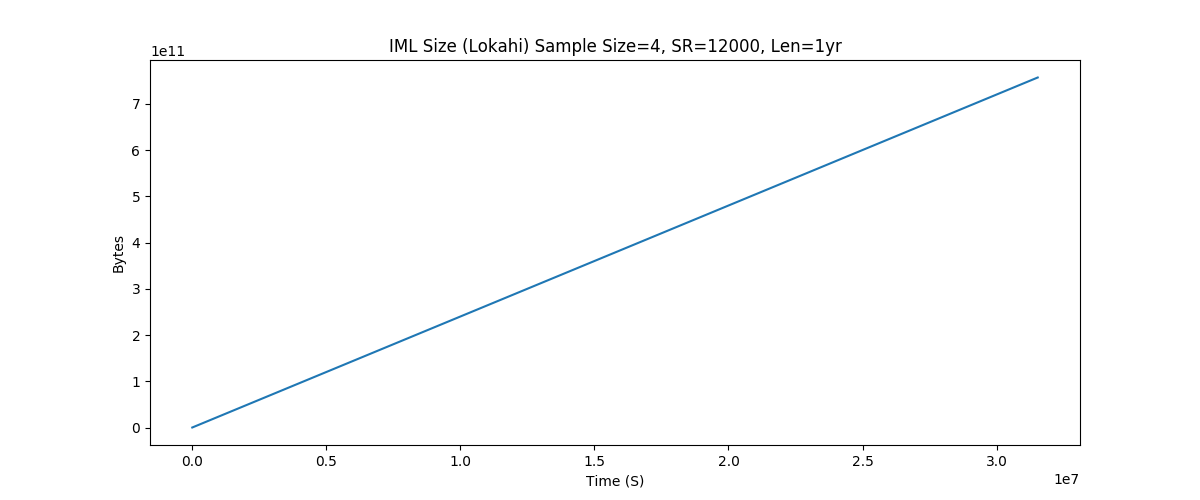
\includegraphics[width=\linewidth]{figures/plot_iml_level_opq.png}
	\caption{IML Growth OPQ}
	\label{fig:iml_growth_opq}
\end{figure}

Figure~\ref{fig:iml_growth_lokahi} shows the IML growth for a single sensor modeled after the Lokahi DSN\@. The Lokahi DSN produces 10 gigabytes of data at 80Hz, 100 gigabytes at 800Hz, and 1000 gigabytes of data at 8000Hz over the course of a year for a single sensor.

\begin{figure}[H]
	\centering
	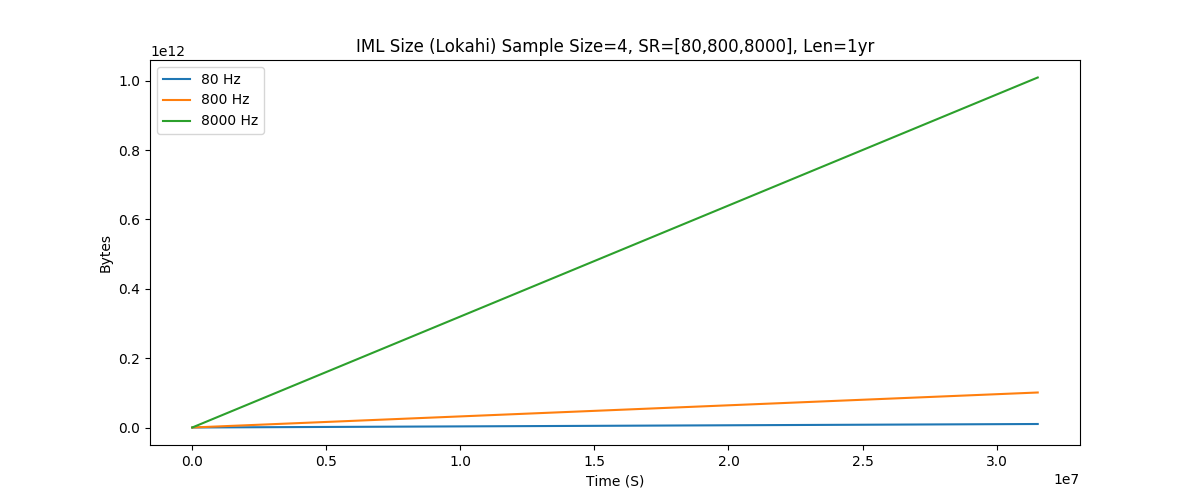
\includegraphics[width=\linewidth]{figures/plot_iml_level_lokahi.png}
	\caption{IML Growth Lokahi}
	\label{fig:iml_growth_lokahi}
\end{figure}

We can estimate upper and lower bounds when the number of sensors recording data to the IML varies over time by examining the mean number of sensors that recorded data $\mu N_{SEN}$ over a time period in seconds $T$.

Equation~\ref{eq:iml:mu_size_iml} provides the calculations for finding the mean size of the IML with varying amounts of sensors.

\begin{equation}\label{eq:iml:mu_size_iml}
	\mu S_{IML} = S_{SAMP} * SR * \mu N_{SEN} * T \pm \delta S_{IML}
\end{equation}

Equations~\ref{eq:iml:e1} and~\ref{eq:iml:e2} provide the error bounds for calculating the mean IML size.

\begin{align}
	\delta N_{SEN} &= \frac{\sigma N_{SEN}}{\sqrt{T}} \label{eq:iml:e1} \\
	\delta S_{IML} &= \delta N_{SEN} * |S_{SAMP} * SR * T| \label{eq:iml:e2}
\end{align}

\paragraph{AML Requirements}
Aggregate measurements provide rolled-up feature extracted values generated from the IML layer. These often include multiple features (i.e. Voltage, Frequency, THD) and descriptive statistics of each feature (i.e. minimum, maximum, average, variance). It's worth noting that the theoretical bounds may differ from the actual bounds in practice due to the way the underlying storage engine persists the values. These differences will be examined in the results section.

Laha allows for multiple sub-levels within the AML. For instance, the OPQ DSN has both measurements and trends AMLs which summarize data at different window lengths. We need to take this into consideration when generating bounds for the AML.

To simplify calculating the bounds on the AML level, we make an assumption that the variance of the size of each AML value is close to 0. The actual metrics for each AML value remain constant sized while the metadata associated with each AML may differ in size. Since each AML value contains similar metadata, the variance on the size of the metadata should remain small.

Equation~\ref{eq:aml_sl} computes the size of a sub-level within the AML $S_{SL}$ by examining the size of an AML entry $S_{V}$, sub-level send rate in Hz $SR$, sensing time in seconds $T$, and a set of sensors $B$.

\begin{equation}\label{eq:aml_sl}
	S_{SL} = S_{V} * SR * T * B_{n}
\end{equation}

Equation~\ref{eq:aml} shows the size of the AML $S_{AML}$ including all sub-levels.

\begin{equation}\label{eq:aml}
	S_{AML} = \sum_{i=1}^{S_{SL_{n}}} S_{SL_{i}}
\end{equation}

Figure~\ref{fig:plot_aml_level_opq_single} examines the growth of the AML level using OPQ as a basis over a time period of one year for a single sensor. We can see that measurements which have a size of 144 bytes and a rate of 1 Hz dominates the data growth which is what we would expect since measurements send at a higher rate. Trends data growth (orange series) on the other hand appears to be almost flat. Finally, the green series represents the total size of the two sub-levels and the sum data storage of the AML for a single sensor.

\begin{figure}[H]
	\centering
	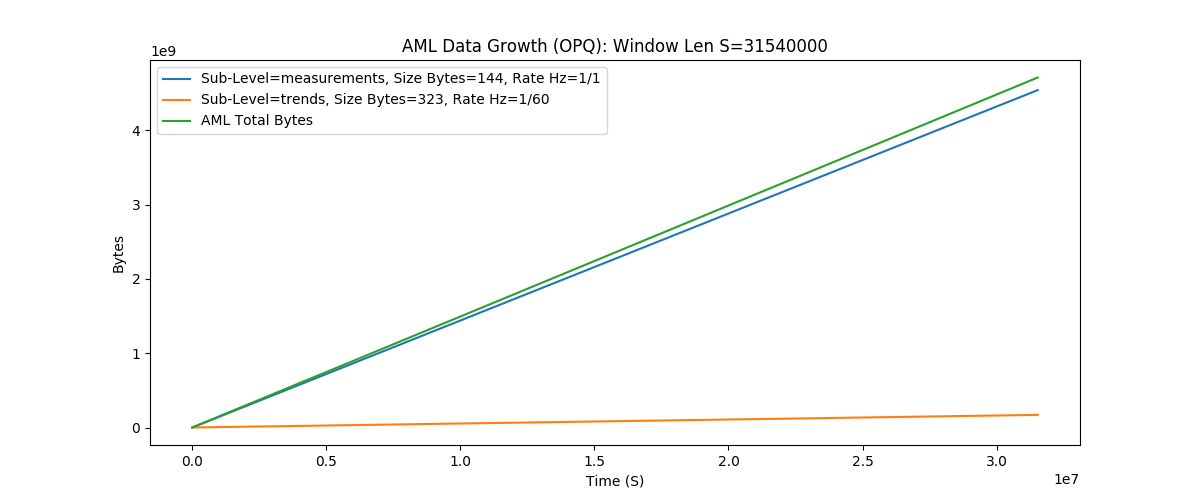
\includegraphics[width=\linewidth]{figures/plot_aml_level_opq_single.png}
	\caption{OPQ AML Growth with Sub-Levels}
	\label{fig:plot_aml_level_opq_single}
\end{figure}

We can see from this figure that left unbounded, the AML can grow to near 5GB a year per sensor in the OPQ network.

Figure~\ref{fig:plot_aml_level_lokahi_single} examines data growth of the AML using Lokahi as a basis over a time period of one year for a single sensor. In this sensor network, the size of each Aggregate Measurement remains constant over each sub-level and only the AML rate varies. We can see that none of the sub-levels tend to dominate.

\begin{figure}[H]
	\centering
	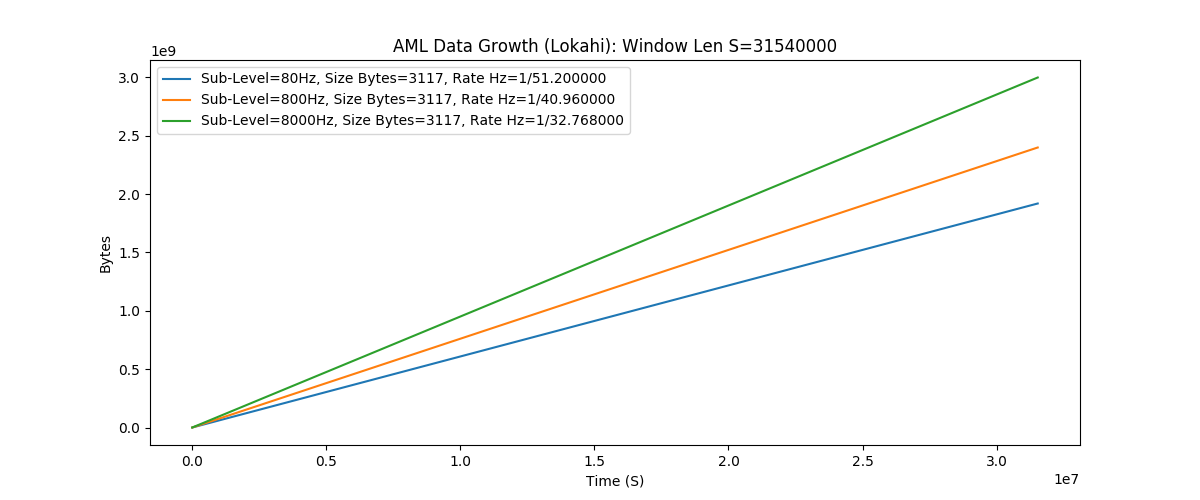
\includegraphics[width=\linewidth]{figures/plot_aml_level_lokahi_single.png}
	\caption{Lokahi AML Growth with Sub-Levels}
	\label{fig:plot_aml_level_lokahi_single}
\end{figure}

From this figure, we can conclude that the AML can grow to a maximum bounds of near 3GB a year per sensor at the maximum sampling rate in the Lokahi network if the data remains unbounded and a minimum of near 2 gigabytes per year per sensor at the lowest sampling rate.

Similar to what was done for the IML, we can estimate bounds assuming the number of sensors sending data is not constant. Equations~\ref{eq:aml:mu_s_sl} and~\ref{eq:aml:mu_s_aml} provide the calculations for mean sub-AML level size and the mean size of the AML respectively.

\begin{align}
	\mu S_{SL} &= S_{V} * SR * T * \mu B \pm \delta S_{SL} \label{eq:aml:mu_s_sl} \\
	\mu S_{AML} &= \sum_{i=1}^{S_{\mu SL_{n}}} \mu S_{SL_{i}} \pm \delta S_{AML} \label{eq:aml:mu_s_aml}
\end{align}

Equations~\ref{eq:aml:e0},~\ref{eq:aml:e1}, and~\ref{eq:aml:e2} provide the error on mean calculations for the AML\@.

\begin{align}
	\delta B &= \frac{\sigma B}{\sqrt{T}} \label{eq:aml:e0} \\
	\delta S_{SL} &= \delta B * |S_{V} * SR * T| \label{eq:aml:e1} \\
	\delta S_{AML} &= \sqrt{\sum_{i=1}^{\delta S_{SL_{n}}}} (\delta S_{SL_{i}}) ^ 2  \label{eq:aml:e2}
\end{align}

\paragraph{DL Requirements}
The detections level contains metadata and associated sampled high fidelity data that was returned from sensors for a given time window. A single detection can contain samples from multiple data streams for a single event of interest.

Similarly to the AML level, we assume that the metadata for each detection remains a constant or close to constant size and we focus on the raw data which dominates the storage requirements in the DL.

I make the assumption that the window lengths for each high-fidelity stream within a single detection are equally sized. In reality, it's possible that a sensor encounters an error and does not return data for the entire requested time window.

Calculating the bounds of this collection is further complicated by the fact that Detections are not generated at a constant rate and the window length of the detections can be highly variable. Further, the number of sensors that return data for any given detection is also variable. Therefore, I provide statistical calculations for these bounds.

First, let's examine calculating the bounds when all parameters are known for a sub-detection. A sub-detection is data returned from a single sensor within a detection. The bounds for each sub-detection is similar to the bounds for a single sensor in the IML, because this level contains the IML data plus some close to constant sized metadata providing context to the IML data.

Equation~\ref{eq:dl:ssd} computes the size of a sub-detection $S_{SD}$ using a given sensor sampling rate in Hz $SR$, the length of the detection in seconds $T$, and the size of the sub-detection metadata $S_{SDM}$.

\begin{equation}\label{eq:dl:ssd}
	S_{SD} = S_{SAMP} * SR * T + S_{SDM}
\end{equation}.

\begin{equation}\label{eq:dl:dl}
	S_{DL} = \sum_{i=0}^{S_{D_{n}}} S_{D_{i}}
\end{equation}

There is a clear upper bound on the size of the DL for a single sensor in the pathological case that the entire data set recorded by a single sensor is one long single Detection. In this pathological case, the upper bounds of the DL is equal to the upper bounds of the IML plus some constant metadata size. The pathological case is not incredibly useful, so, let's look at this from a statistical standpoint.

We can provide estimated bounds on the DL with an estimated data rate $\mu DR$ which provides the mean number of bytes generated per second within the DL\@. It should be noted that this includes the parameters for all sub-detections as well. The calculation for the mean size of the DL is given in Equation~\ref{eq:dl:mu_s_dl}.

\begin{equation}\label{eq:dl:mu_s_dl}
	\mu S_{DL} = \mu DR * T \pm \delta S_{DL}
\end{equation}

The errors for the mean size of the DL are given in Equations~\ref{eq:dl:e0} and~\ref{eq:dl:e1}.

\begin{align}
	\delta DR = \frac{\sigma DR}{\sqrt{T}} \label{eq:dl:e0} \\
	\delta S_{DL} = \delta {DR} * |T| \label{eq:dl:e1}
\end{align}

Let's next compare the estimated sizes of the DL for the OPQ and Lokahi networks using statistics gathered for these networks. Table~\ref{table:estimated_mu_dr} provides the parameters used for these comparisons.

\begin{table}[H]
	\centering
	\caption{Estimated $DR$}
	\begin{tabularx}{\textwidth}{lll}
		\toprule
		\textbf{Network} & $\bm{\mu DR}$ & $\bm{\sigma DR}$ \\
		\midrule
		OPQ & 13064.9 & 200712.1 \\
		Lokahi & 0.0 & 0.0 \\
		\bottomrule
	\end{tabularx}
	\label{table:estimated_mu_dr}
\end{table}

Figure~\ref{fig:plot_dl_opq_avg} shows the estimated size for the DL on the OPQ network. The errors are small enough that they are not discernible in this plot. Over a period of one year, the DL is expected to grow to 383 gigabytes $\pm$ 1.05 gigabytes.

\begin{figure}[H]
	\centering
	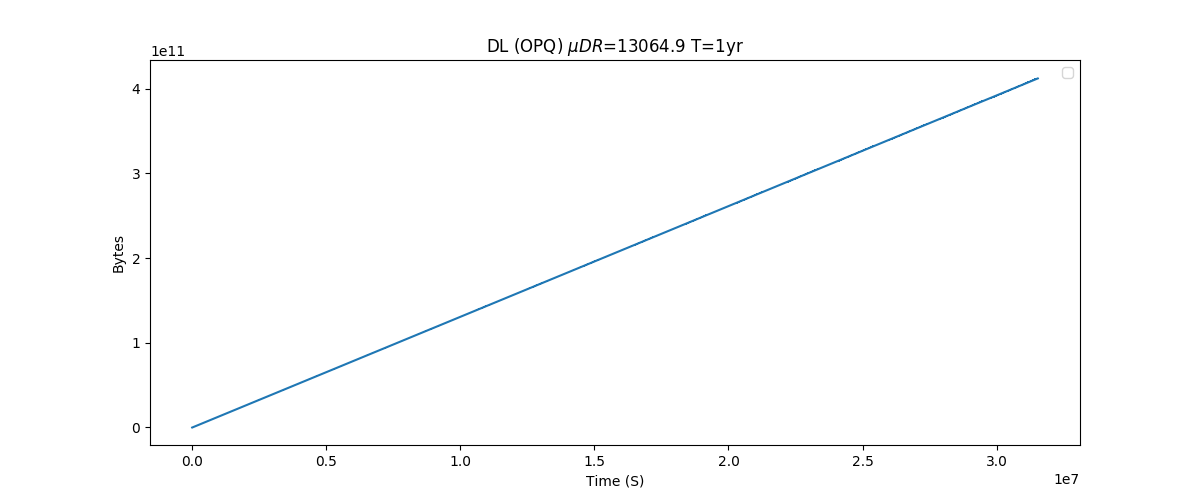
\includegraphics[width=\linewidth]{figures/plot_dl_opq_avg.png}
	\caption{Estimated OPQ DL}
	\label{fig:plot_dl_opq_avg}
\end{figure}

\paragraph{IL Requirements}
The Incidents Level provides added context on top of the DL in the form of signal of interest classifications. This level is structured similarly to the DL in that it contains trimmed down IML samples from one or more sensors over a varying time window and added context in the form of metadata. Due to these similarities, the bounds calculations are also quite similar.

The IL differs from the DL in that the associated IML samples in the IL are always subsets of the samples in the DL\@. The IL also differs from the DL in the fact that the IL does not have a concept of ``sub-incidents". Every Incident in the IL is associated with exactly one Event waveform.

When all parameters are known, the individual size of an Incident $S_{I}$ within the IL can be calculated over the size of each sample $S_{SAMP}$, sample rate in Hz $SR$, length of the incident $T+{I}$, and size of the associated metadata $S_{M}$ with Equation~\ref{eq:il:s_i}.

\begin{equation}\label{eq:il:s_i}
	S_{I} = S_{SAMP} * SR * T_{I} + S_{M}
\end{equation}

Then, computing the size of the entire IL can be done with a simple summation as shown in Equation~\ref{eq:il:s_il}.

\begin{equation}\label{eq:il:s_il}
	S_{IL} = \sum_{i=0}^{S_{I_{n}}} S_{I_{i}}
\end{equation}

There is a clear upper bound on the size of the IL for a single sensor in the pathological case that the entire data set recorded by a single sensor is one long single Incident. In this pathological case, the upper bounds of the IL is equal to the upper bounds of the IML plus some constant metadata size. The pathological case is not incredibly useful, so, let us look at this from a statistical standpoint.

We can provide estimated bounds on the IL assuming a mean Incident rate in bytes per second $\mu IR$ as shown in Equation~\ref{eq:il:mu_s_il}.

\begin{equation}\label{eq:il:mu_s_il}
 \mu S_{IL} = \mu IR * T \pm \delta S_{IL}
\end{equation}

Equations~\ref{eq:il:e0} and~\ref{eq:il:e1} provide error bounds on the estimated size of the IL\@.

\begin{align}
	\delta IR &= \frac{\sigma IR}{\sqrt{T}} \label{eq:il:e0} \\
	\delta S_{IL} &= \delta IR * |T| \label{eq:il:e1}
\end{align}

Let us next compare the estimated sizes of the IL for the OPQ and Lokahi networks using statistics gathered for these networks. Table~\ref{table:estimated_mu_ir} provides the parameters used for these comparisons.

\begin{table}[H]
	\centering
	\caption{Estimated $IR$}
	\begin{tabularx}{\textwidth}{lll}
		\toprule
		\textbf{Network} & $\bm{\mu DR}$ & $\bm{\sigma DR}$ \\
		\midrule
		OPQ & 49.1 & 1942.5 \\
		Lokahi & 0.0 & 0.0 \\
		\bottomrule
	\end{tabularx}
	\label{table:estimated_mu_ir}
\end{table}

Figure~\ref{fig:plot_il_opq_avg} shows the estimated size for the IL on the OPQ network. The errors are small enough that they are not discernible in this plot. Over a period of one year, the IL is expected to grow to 1.44 gigabytes $\pm$ 0.01 gigabytes.

\begin{figure}[H]
	\centering
	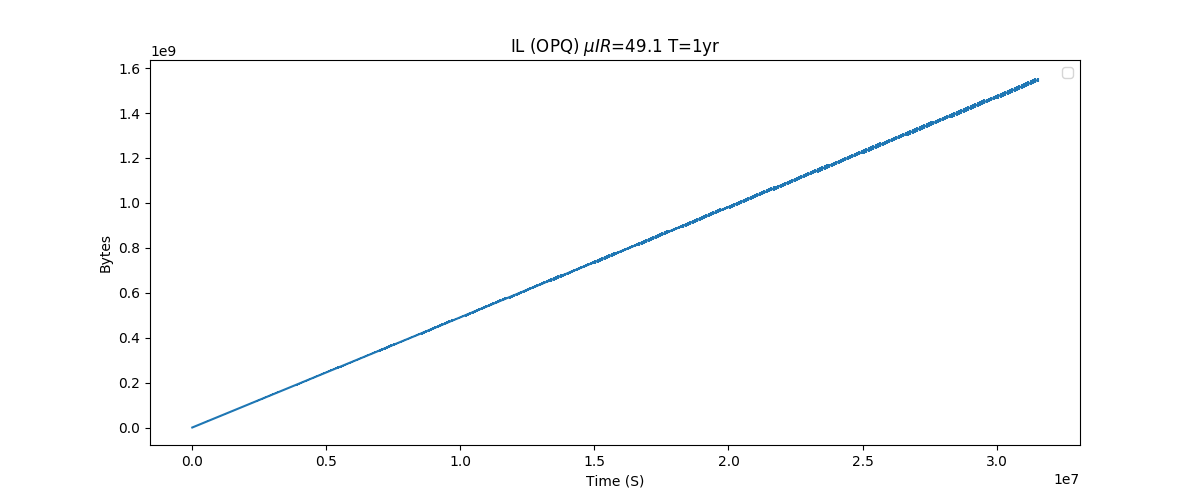
\includegraphics[width=\linewidth]{figures/plot_il_opq_avg.png}
	\caption{Estimated OPQ IL}
	\label{fig:plot_il_opq_avg}
\end{figure}

\paragraph{PL Requirements}
The Phenomena Level provides actionable insights and context beyond what is provided in the IL. Examples of added context include predictive analysis, Annotations, or similarity metrics between Incidents. The Phenomena level consists mainly of metadata describing the Phenomena. Different types of Phenomena require varying amounts of metadata.

Equation~\ref{eq:pl} calculates the size of the PL $S_{PL}$ by summing the size of each Phenomena $S_{P}$ that is stored.

\begin{equation}\label{eq:pl}
	S_{PL} = \sum_{i=0}^{S_{P_{n}}} S_{P_{i}}
\end{equation}

\paragraph{Comparing Laha Requirements}

Now that we can compute the bounds for different levels within the Laha hierarchy, let's examine how the requirements compare between each level given data that resembles the OPQ and Lokahi DSNs.

Analytically, when all parameters are known, the size of the entire DSN $S_{DSN}$ can be computed as shown in Equation~\ref{eq:s_dsn}.

\begin{equation}\label{eq:s_dsn}
	S_{DSN} = S_{IML} + S_{AML} + S_{DL} + S_{IL} + S_{P}
\end{equation}

Statistically speaking, the mean size and error of the entire DSN are provided by Equations~\ref{eq:dsn:mu_s_dsn} and~\ref{eq:dsn:e} respectively.

\begin{align}
	\delta S_{DSN} &= \sqrt{(\delta S_{IML})^2 + (\delta S_{AML})^2 + (\delta S_{DL})^2 + (\delta S_{IL})^2 + (\delta S_{P})^2} \label{eq:dsn:e} \\
	\mu S_{DSN} &= \mu S_{IML} + \mu S_{AML} + \mu S_{DL} + \mu S_{IL} + \mu S_{P} \pm \delta S_{DSN} \label{eq:dsn:mu_s_dsn}
\end{align}

First, let's look at the size of Laha with parameters estimated from OPQ. The estimated parameters for this scenario are given in Table~\ref{table:estimated_laha_opq}.

\begin{table}[H]
	\centering
	\caption{OPQ Estimated Parameters}
	\begin{tabularx}{\textwidth}{lll}
		\toprule
		\textbf{Field} & \textbf{Mean} & \textbf{Stddev} \\
		\midrule
		$S_{SAMP}$ & 2 & 0.0 \\
		$SR$ & 12000 & 0.0 \\
		$S_{MEASUREMENT}$ & 145 & 0.0 \\
		$R_{MEASUREMENT}$ & 1 & 0.0 \\
		$S_{TREND}$ & 324 & 0.0 \\
		$R_{TREND}$ & $\frac{1}{60}$ & 0.0 \\
		$\mu N_{SEN}$ & 9.9 & 0.7 \\
		$\mu DR$ & 13064.0 & 200712.1 \\
		$\mu IR$ & 49.1 & 1942.5 \\
		\bottomrule
	\end{tabularx}
	\label{table:estimated_laha_opq}
\end{table}

Figure~\ref{fig:plot_lala_opq} shows the bounds of the entire network.

\begin{figure}[H]
	\centering
	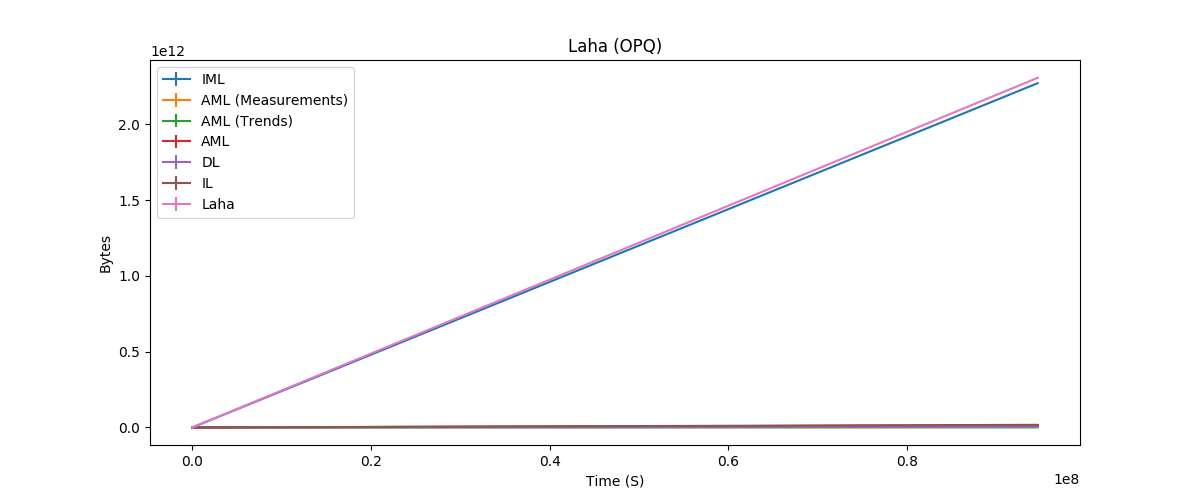
\includegraphics[width=\linewidth]{figures/plot_laha_opq.png}
	\caption{Estimated Laha (OPQ)}
	\label{fig:plot_lala_opq}
\end{figure}

We can gather that the bounds on the entire OPQ network given estimated parameters from the network are 7953 gigabytes $\pm$ 1.1 gigabytes per year. It's clear that the IML provides most of this data. We can also see that over time, the DL dominates all other levels except the IML.

By representing the data as a pie chart (Figure~\ref{fig:plot_lala_opq_pie}), we can gain a better understanding of how these levels compare at the end of a year. The first (left most) pie chart shows that the IML dominates the overall data size. This makes sense because this level represents raw samples which is always going to be the largest set of data.

By removing the IML from the results, the second pie chart (right most) shows how the other levels compare to each other. From this, we can gather that the DL is the next largest. This makes sense because the DL represents windows of samples that may or may not include Incidents, and therefore the DL should always be larger than the IL which is essentially the DL with further filtering and classification.

We also observe that the size of the AML also takes up the next largest percentage of space. This is mainly due to the fact that OPQ collects aggregate measurements once per second. Left unbounded, this collection can become quite sizable.

\begin{figure}[H]
	\centering
	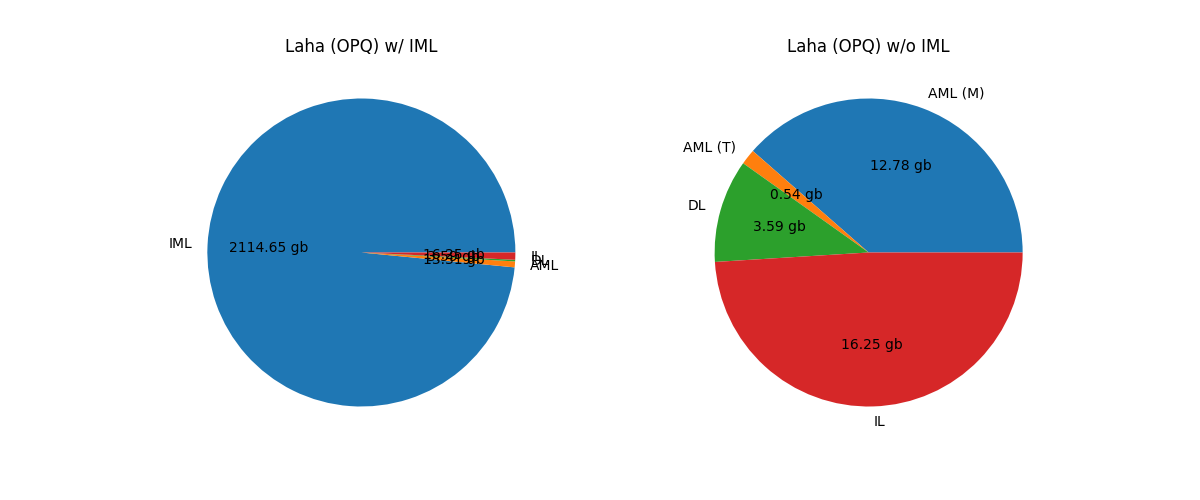
\includegraphics[width=\linewidth]{figures/plot_laha_opq_pie.png}
	\caption{Estimated Laha (OPQ)}
	\label{fig:plot_lala_opq_pie}
\end{figure}

Finally, we summarize the results in Table~\ref{table:summarized_laha_results_opq}.

\begin{table}[H]
	\centering
	\caption{Summarized Laha Results (OPQ)}
	\begin{tabularx}{\textwidth}{lll}
		\toprule
		\textbf{Laha Level} & \bm{$\mu Size$} \textbf{GB} & \bm{$\delta Size$} \textbf{GB} \\
		\midrule
		IML & 6978.36 & 0.08 \\
		AML (Measurements) & 42.16 & 0.0005 \\
		AML (Trends) & 1.57 & 0.00002 \\
		AML (Total) & 43.73 & 0.0005 \\
		DL & 383.69 & 1.05 \\
		IL & 1.44 & 0.01 \\
		PL & NA & NA \\
		Laha (Total) & 7407.22 & 1.05 \\
		\bottomrule
	\end{tabularx}
	\label{table:summarized_laha_results_opq}
\end{table}

\subsubsection{Evaluation of TTL}

During the acquisition and curating of data, metrics were collected and stored about how much data is saved (in bytes) versus how much data is discarded at each level within the Laha data hierarchy. These numbers were compared against data storage as if the OPQ and Lokahi frameworks were to take a ``store everything" approach. Evaluation metrics provided include percentage of data storage saved per data hierarchy level as well as an estimate of overall decrease in data storage requirements for the entire DSN. A positive result from these metrics would show significant reduction in storage requirements for each level in the framework compared against a ``store everything approach" and other state-of-the-art data storage solutions.

I also provide metrics on ``continuous storage pressure" which is a measure of the average amount of data storage required at each level given the current state of the network. That is, since data at all lower levels of the framework assigns a TTL to the data within the collection, the collection will exhibit a constant data pressure during sensor data collection. For example, at the lowest level, the IML collects raw data from all sensors all the time. Given the sample rate per sensor, the size per sample, the number of sensors, and a known TTL for this level, I can estimate the maximum bounds of data management requirements that the IML requires. We can develop similar estimation strategies with higher levels of the framework. I computed the statistical error between the predicted storage pressure and the actual storage pressure recorded during the experiments. A positive outcome would show strong correlation between the predicted storage pressure and the actual storage pressure. A negative outcome would show weak correlation between the predicted and actual values.

\subsubsection{Combined Evaluation of Tiered Data Management}
Finally, I provided an evaluation that weighs the results of all three metrics against each other. For example, if I see positive results for data storage reduction and negative results for false positives, do the benefits of the data storage reduction outweigh the negatives of increased false positives?

I expect that DSNs that have a lower signal-to-noise ratio will see greater benefits from tiered data management than DSNs that already have a decent signal-to-noise ratio.

\section{Evaluation of Tertiary Goals}\label{sec:evaluation-of-tertiary-goals}
In order to achieve the main goals of this framework, I claim that either all or a subset of the following tertiary goals must be fulfilled. Optimization of triggering, detection, classification, sensor energy usage, bandwidth, predictive analytics, and the ability to derive models of the underlying sensing field topology.

To evaluate these tertiary goals, I selected and implemented DSN optimization techniques from current literature. I then compared and contrasted the usefulness of different techniques and discuss how each of these techniques perform in the different sensor domains.

Finally, I discuss how each of these tertiary goals make progress towards overall goals of this sensor network.

\subsection{Evaluation of Adaptive Optimizations for Triggering}\label{subsec:evaluation-of-adaptive-optimizations-for-triggering}
Triggering is the act of observing a feature extracted data stream for interesting features and triggering sensors to provide raw data for a requested time window for higher level analysis. Adaptively optimizing triggering is a way to tune triggering algorithms and parameters with the aim of decreasing false positives and false negatives. In this context, a false positive is triggering on a data stream that does not contain a signal of interest and a false negative is not triggering on a data stream that does contain a signal of interest.

Adaptive triggering is only useful in networks that utilize triggering. Specifically, this technique can not be applied to DSNs that take a collect everything all the time approach.

Triggering can also have significant impacts on overall sensor power requirements and DSN bandwidth requirements. Many of the optimizing triggering algorithms present in the literature exist to minimize sensor energy requirements and bandwidth requirements. This is addressed in great detail in the literature review by Anastasi et al. \cite{anastasi_energy_2009}. This is accomplished by reducing communications between sensor nodes and the sink. It's argued in \cite{pottie2000wireless} that the cost of transmitting a single bit of information from a sensor cost approximately the same as running 1000 operations on that sensor now. However, there is some contention on this topic as \cite{alippi_adaptive_2010} argues that in some modern sensors computational requirements can equal or eclipse those of  sensor communication.

Even if a DSN utilizes triggering, it's not clear that adaptive triggering even takes place. The first question I evaluated is, does adaptive optimization of triggering take place at all given the domain of the DSN? That is, does the nature of the underlying sensor field contribute to optimization of triggering? I compared if and how optimizations take place in the two reference networks for the domains of PQ and infrasound.

In order to evaluate triggering efficiency within our Laha deployments, Laha only adaptively modifies triggering for half of the devices in the OPQ deployment. In the Lokahi deployment, I  ran the same experiment twice. The first run did not optimize triggering and the second run did optimize triggering.

Once the experiments were run, I first determined if optimization of triggering has occurred, and if it did, compared the number of false negatives and false positives against the runs that did not use optimized triggering or where optimization did not occur.

I hope to show that a side effect of Laha's optimized triggering is reduced bandwidth and sensor energy requirements. To this end, I calculated metrics for total data sent and received at the sink node of each network for each device in the network. A positive result would show decreased bandwidth usage for devices that utilize optimized triggering. A negative result would show similar or more bandwidth usage for devices that utilize optimized triggering.

I further hope to show that another benefit of Laha's optimized triggering is reduced sensor energy requirements. The evaluation for this metric occurred with the Lokahi network where sensors can be dependent on batteries. I ran two experiments. For each experiment, all sensors were charged to battery level of 100\%. In the first experiment, I did not utilize optimized triggering. In the second experiment I did utilize optimized triggering. In both experiments, I measured the final battery level after the experiment and also measure how quickly the battery depletes for each sensor. This is possible because data in the Lokahi network contains timestamped entries with battery levels.

\subsection{Evaluation of Adaptive Optimizations for Detection and Classifications}\label{subsec:evaluation-of-adaptive-optimizations-for-detection-and-classifications}
Detections occur when triggering observes something ``interesting" in the feature extracted data stream. A Detection is a contiguous window of raw sensor data that was requested by triggering that may or may not contain signals of interest. Optimizing detections involves optimized the window sizes to increase the signal-to-noise ratio of the window. Fine grained features are then computed by Detection Actors and moved to the Incidents Level where classification of signals takes place. Optimizing Detections involves trimming detection windows to increase signal-to-noise. Optimizing of classifications for Incidents involves tuning parameter sets for the underlying classification algorithms.

Predictive and Locality Phenomena as well as topology optimizations were used to provide optimizations to the Detections and Incidents levels.

Evaluation of adaptive optimizations for detection and classification within the Laha network were conducted differently for each Laha deployment.

In the Lokahi deployment, I controlled the production of infrasound signals using the available infrasound source. I ran two experiments, where the amplitudes and frequencies of the signals are the same and the locations of the devices remain invariant. In the first experiment, Laha did not use optimized detection or classification provided by Phenomena. In the second experiment, Laha did use optimized detection and classification techniques provided by Phenomena.

With known frequencies and amplitudes of the infrasound signals, I can compare the rate of detections and classifications between the optimized and unoptimized experimental runs. I expect to see a greater number of and more accurate detections and classifications from the optimized experiment.

In the OPQ deployment, I compared the same metrics as the Lokahi deployment, but instead of controlling the source signal, I co-located OPQBoxes with industry standard meters. In each pair of co-located OPQBoxes, one was analyzed using Phenomena optimized detection and classification algorithms and the other was analyzed using unoptimized detection and classification algorithms.

I collected and evaluated the number of false positives and false negatives for Incidents generated with optimization and without optimization. A positive outcome would include a decrease in either false positives, false negatives, or both. A negative result would be an increase in either or both false positives or false negatives.

I also calculated the signal-to-noise ratio in Detections to determine if optimization of detections is working. A positive outcome is an increase in the signal-to-noise ration and a negative outcome would be similar or a decrease in signal-to-noise ratio.

\subsection{Evaluation of Model of Underlying Sensor Field Topology}
Laha should be able to build a model of the underlying sensing field topology. This is not the topology of the physical layout of the sensors (this is generally already known a priori or by collecting location information), but rather the topology by which signals travel. For example, in a PQ network the topology is the physical power grid and switches that PQ signals travel through. In an infrasound network, the topology is the atmosphere through which sound waves travel. Laha aims to build a statistical model of the distances between sensors according to the topology of the sensing field by observing recurrent incidents over time. This can perhaps shed some light on understanding the topology of a sensing field without knowing anything about it before hand.

Much of the literature on topology management is written to decrease sensor energy requirements by exploiting the density of sensors within a sensing field topology. For example, the ASCENT\cite{cerpa2004ascent} framework provides adaptive self configuring sensors that exploit topology denseness to decrease sensor energy usage. Several other frameworks have been designed with the same goal of reducing energy usage by exploiting topology\cite{schurgers2002stem},\cite{schurgers2002topology}.

To evaluate the model of the sensing field topology, I took two different approaches for each Laha deployment. In both deployment, the sensing field topology is known beforehand to provide a ground truth. I then compared Laha's computed signal distance between sensors to the actual signal distance between sensors as provided by the ground truths.

In the Lokahi deployment, sensors were strategically placed at different distances from an infrasound source. Some sensors were close to each other geographically, but separated by terrain that infrasound signals could not easily travel through. By moving the infrasound source, I can expect to see infrasound signals arriving or not arriving at the sensors depending on the source and direction of the signal along with the physical features of the land. By performing multiple experiments, I provided a model of the physical environment topology that Laha has built. I compared Laha's model to the known topology and provide a statistical error analysis.

In the OPQ deployment, sensors were strategically placed on like and unlike electrical lines to observe how distributed PQ signals move through a power grid. In this deployment, Laha built a topology model that doesn't show physical geographic distance between sensors, but instead built a model of the electrical distance between sensors. This data was evaluated by comparing the electrical distances found by the Laha model to the actual UH power grid as referenced by the schematic provided by the Office of Energy Management at UH Manoa. A statistical error analysis of the differences between electrical distances between the model and the schematic is provided as an evaluation metric.

A positive outcome would be to show that there is high correlation between the Laha signal distances and the ground truth distances. A negative outcome would show low correlation.

Assuming high correlation and a statistical model of the sensing field, I evaluated if Laha is able to use this information to optimize triggering, classification, or predictive analytics. In order to evaluate this, I collected the number of false positives and false negatives at all levels in the Laha hierarchy while optimizing from topology and without optimizing from topology. I expect to see less false positives and less false negatives when utilizing topology optimizations. A negative result would be a larger number of false positives or false negatives.

I expect to only see results in networks where signals travel fast enough to create a statistical difference between arrival times at the various sensors. In sensing fields where signals travel slowly and uniformly (i.e. a temperature collection DSN), it may be more difficult or impossible to actually determine the sensing field topology.
